\subsection{Solving XKCD 287 using Z3}

\begin{figure}[H]
\centering
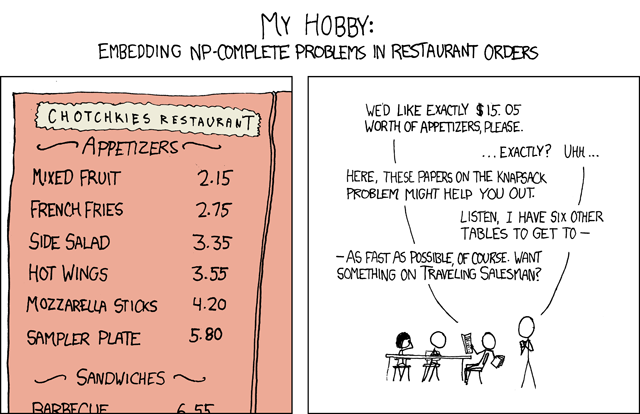
\includegraphics[scale=7]{SMT/xkcd287/np_complete.png}
\caption{xkcd \#287}
\end{figure}

( \url{https://www.xkcd.com/287/} )

The problem is to solve the following equation:
$2.15a + 2.75b + 3.35c + 3.55d + 4.20e + 5.80f == 15.05$,
where a..f are integers.
So this is a linear diophantine equation.

\begin{lstlisting}
#!/usr/bin/python

from z3 import *

a,b,c,d,e,f = Ints('a b c d e f')
s = Solver()
s.add(215*a + 275*b + 335*c + 355*d + 420*e + 580*f == 1505, a>=0, b>=0, c>=0, d>=0, e>=0, f>=0)

results=[]

# enumerate all possible solutions:
while True:
    if s.check() == sat:
        m = s.model()
        print m
        results.append(m)
        block = []
        for d in m:
            c=d()
            block.append(c != m[d])
        s.add(Or(block))
    else:
        print "results total=", len(results)
        break
\end{lstlisting}

( The source code: \url{https://github.com/DennisYurichev/SAT_SMT_article/blob/master/SMT/xkcd287/xkcd287.py} )

There are just 2 solutions:

\begin{lstlisting}
[f = 0, b = 0, a = 7, c = 0, d = 0, e = 0]
[f = 1, b = 0, a = 1, c = 0, d = 2, e = 0]
results total= 2
\end{lstlisting}

Wolfram Mathematica can solve the equation as well:

\begin{lstlisting}
In[]:= FindInstance[2.15 a + 2.75 b + 3.35 c + 3.55 d + 4.20 e + 5.80 f == 15.05 && 
	a >= 0 && b >= 0 && c >= 0 && d >= 0  && e >= 0 && f >= 0, 
	{a, b, c, d, e, f}, Integers, 1000]

Out[]= {{a -> 1, b -> 0, c -> 0, d -> 2, e -> 0, f -> 1},
	{a -> 7, b -> 0, c -> 0, d -> 0, e -> 0, f -> 0}}
\end{lstlisting}

1000 means ``find at most 1000 solutions'', but only 2 are found.
See also: \url{http://reference.wolfram.com/language/ref/FindInstance.html}.\\
\\
Other ways to solve it:
\url{https://stackoverflow.com/questions/141779/solving-the-np-complete-problem-in-xkcd},
\url{http://www.explainxkcd.com/wiki/index.php/287:_NP-Complete}.

